
\subsection{Answers}
\begin{table}[htb]%
\begin{center}%
\caption{Q26: Is MPI providing all the communication semantics required by your application? If not, what is missing?}%
\label{tab:Q26-ans}%
\begin{tabular}{l|l|r}%
\hline%
Choice & Abbrv. & \# Answers \\%
\hline%
{\small MPI is providing all the communication s$\cdots$} & MPI provides all & 248 (33.8\%) \\%
{\small Additional optimization opportunities in$\cdots$} & Additional opt & 182 (24.8\%) \\%
Resilience (fault tolerance) & Resilience & 163 (22.2\%) \\%
{\small Latency hiding (including asynchronous c$\cdots$} & Latency hiding & 156 (21.3\%) \\%
{\small Another API which is easier and/or simpl$\cdots$} & Another API & 115 (15.7\%) \\%
Endpoints (multi-thread, sessions) & End-points & 93 (12.7\%) \\%
other & - & 46 (6.3\%) \\%
\hline%
\multicolumn{2}{c}{total} & 1003 (733)\\%
\hline%
\end{tabular}%
\end{center}%
\end{table}%

\clearpage%
{\footnotesize\begin{landscape}%
\begin{longtable}[htb]{r|c|c|c|c|c|c|c|c|c|c}%
\caption{Q26: Is MPI providing all the communication semantics required by your application? If not, what is missing?}%
\label{tab:Q26-mans} \\%
\hline%
Multi-Answer & overall & FR & GR & IT & UK & eu & JP & RU & US & others \\
 \hline%
\endfirsthead%
\multicolumn{11}{r}{(continued from the previous page)}\\%
\hline%
Multi-Answer & overall & FR & GR & IT & UK & eu & JP & RU & US & others \\
 \hline%
\endhead%
\hline%
(total) & 733 & 104 & 135 & 48 & 57 & 117 & 60 & 86 & 52 & 74 \\%
\hline%
\multicolumn{11}{r}{(continue to the next page)}\\%
\endfoot%
\hline%
(total) & 733 & 104 & 135 & 48 & 57 & 117 & 60 & 86 & 52 & 74 \\%
\hline%
\endlastfoot%
\hline%
{MPI provides all} & 234 & 27 & 54 & 19 & 22 & 31 & 11 & 42 & 12 & 16 \\%
{Additional opt} & 72 & 12 & 12 & 3 & 2 & 9 & 7 & 8 & 3 & 16 \\%
{Resilience} & 61 & 12 & 14 & 4 & 4 & 5 & 5 & 7 & 4 & 6 \\%
{Latency hiding} & 61 & 10 & 9 & 4 & 0 & 15 & 7 & 6 & 4 & 6 \\%
{Another API} & 56 & 10 & 6 & 5 & 3 & 10 & 7 & 6 & 2 & 7 \\%
{End-points} & 33 & 3 & 4 & 5 & 2 & 3 & 4 & 2 & 4 & 6 \\%
{Resilience, Additional opt} & 29 & 2 & 7 & 3 & 2 & 9 & 1 & 2 & 3 & 0 \\%
{Latency hiding, Additional opt} & 21 & 1 & 5 & 0 & 1 & 3 & 5 & 2 & 1 & 3 \\%
{Latency hiding, Resilience} & 12 & 5 & 3 & 0 & 1 & 0 & 1 & 0 & 2 & 0 \\%
{End-points, Additional opt} & 10 & 1 & 2 & 0 & 1 & 1 & 1 & 1 & 3 & 0 \\%
{Latency hiding, Resilience, Additional opt} & 9 & 2 & 1 & 0 & 1 & 4 & 0 & 0 & 0 & 1 \\%
{Latency hiding, End-points} & 9 & 1 & 1 & 0 & 1 & 3 & 1 & 1 & 1 & 0 \\%
{Latency hiding, End-points, Resilience} & 8 & 2 & 1 & 0 & 0 & 0 & 1 & 0 & 1 & 3 \\%
{Resilience, Another API} & 8 & 2 & 0 & 0 & 0 & 5 & 0 & 0 & 1 & 0 \\%
{Another API, MPI provides all} & 7 & 3 & 1 & 0 & 0 & 1 & 1 & 0 & 0 & 1 \\%
{Latency hiding, End-points, Resilience, Another API} & 7 & 0 & 0 & 0 & 7 & 0 & 0 & 0 & 0 & 0 \\%
{Latency hiding, Another API} & 6 & 0 & 2 & 0 & 1 & 1 & 0 & 0 & 1 & 1 \\%
{Resilience, Additional opt, Another API} & 6 & 1 & 1 & 1 & 1 & 0 & 0 & 2 & 0 & 0 \\%
{Additional opt, Another API} & 5 & 0 & 0 & 0 & 0 & 1 & 0 & 1 & 1 & 2 \\%
{End-points, Resilience, Additional opt} & 5 & 1 & 0 & 0 & 1 & 0 & 2 & 0 & 1 & 0 \\%
{Latency hiding, End-points, Resilience, Additional opt} & 4 & 1 & 0 & 0 & 0 & 0 & 1 & 1 & 0 & 1 \\%
{Latency hiding, Resilience, Additional opt, Another API} & 3 & 1 & 0 & 0 & 1 & 1 & 0 & 0 & 0 & 0 \\%
{End-points, Resilience} & 3 & 1 & 0 & 0 & 0 & 1 & 0 & 0 & 1 & 0 \\%
{End-points, Another API} & 3 & 1 & 1 & 0 & 0 & 0 & 0 & 0 & 0 & 1 \\%
{Latency hiding, End-points, Additional opt} & 2 & 0 & 0 & 1 & 0 & 1 & 0 & 0 & 0 & 0 \\%
{Good integration with modern C++, including coroutines/fibers/async/future as well as object (de)serialization} & 2 & 0 & 0 & 0 & 0 & 0 & 0 & 0 & 2 & 0 \\%
{I do not know} & 2 & 1 & 0 & 0 & 0 & 1 & 0 & 0 & 0 & 0 \\%
{Additional opt, MPI provides all} & 2 & 0 & 1 & 0 & 0 & 1 & 0 & 0 & 0 & 0 \\%
{Latency hiding, Resilience, Another API} & 2 & 0 & 1 & 0 & 0 & 1 & 0 & 0 & 0 & 0 \\%
{Another API, Exception handling} & 1 & 0 & 1 & 0 & 0 & 0 & 0 & 0 & 0 & 0 \\%
{Latency hiding, Additional opt, Another API} & 1 & 0 & 1 & 0 & 0 & 0 & 0 & 0 & 0 & 0 \\%
{Latency hiding, Additional opt, notified access} & 1 & 0 & 0 & 0 & 0 & 1 & 0 & 0 & 0 & 0 \\%
{Latency hiding, A better interaction with OpenMP tasks} & 1 & 1 & 0 & 0 & 0 & 0 & 0 & 0 & 0 & 0 \\%
{Resilience, MPI provides all} & 1 & 0 & 0 & 1 & 0 & 0 & 0 & 0 & 0 & 0 \\%
{Latency hiding, End-points, Need a way to tell when processes first go out of sync.} & 1 & 0 & 1 & 0 & 0 & 0 & 0 & 0 & 0 & 0 \\%
{QOS by communicator - I know which traffic I wish to prioritise from a latency perspective!} & 1 & 0 & 0 & 0 & 1 & 0 & 0 & 0 & 0 & 0 \\%
{Latency hiding, Additional opt, One sided with completation signal (see OpenSHMEM)} & 1 & 0 & 0 & 0 & 1 & 0 & 0 & 0 & 0 & 0 \\%
{Additional opt, Another API, Accelerator triggered communication} & 1 & 0 & 0 & 0 & 0 & 0 & 0 & 0 & 1 & 0 \\%
{Resilience, Additional opt, Another API, MPI provides all} & 1 & 0 & 0 & 0 & 0 & 0 & 0 & 0 & 0 & 1 \\%
{Latency hiding, End-points, Resilience, Additional opt, Another API} & 1 & 0 & 0 & 1 & 0 & 0 & 0 & 0 & 0 & 0 \\%
{RPC like API} & 1 & 1 & 0 & 0 & 0 & 0 & 0 & 0 & 0 & 0 \\%
{Debugging capabilities, i.e. message sequence traces, type matching, etc.} & 1 & 0 & 0 & 0 & 0 & 0 & 0 & 1 & 0 & 0 \\%
{Latency hiding, End-points, Another API} & 1 & 0 & 0 & 0 & 0 & 0 & 1 & 0 & 0 & 0 \\%
{Too stupid to give an educated opinion} & 1 & 0 & 0 & 0 & 0 & 0 & 0 & 1 & 0 & 0 \\%
{Latency hiding, End-points, Expose de-aggregated (eg Request-based) REMOTE completion for individual MPI\_PUT operations. Allow Accumulate/Fetch-op to concurrently perform different computational operations on a single location (eg fetch-add racing with swap or compare-swap)} & 1 & 0 & 0 & 0 & 0 & 0 & 0 & 0 & 1 & 0 \\%
{RPC, reasons mentioned above.} & 1 & 0 & 0 & 0 & 0 & 0 & 0 & 0 & 1 & 0 \\%
{client-server connection for coupled application, more versatility in launching multiple applications in parallel than MPMD} & 1 & 0 & 0 & 0 & 0 & 0 & 0 & 0 & 0 & 1 \\%
{Resilience, Additional opt, Possibility to dynamically change the communicators topology upon machine failure or addition} & 1 & 1 & 0 & 0 & 0 & 0 & 0 & 0 & 0 & 0 \\%
{Don't know} & 1 & 0 & 0 & 0 & 0 & 0 & 0 & 1 & 0 & 0 \\%
{load balancing} & 1 & 0 & 0 & 0 & 0 & 1 & 0 & 0 & 0 & 0 \\%
{Latency hiding, End-points, Additional opt, Another API} & 1 & 0 & 0 & 0 & 0 & 0 & 0 & 1 & 0 & 0 \\%
{Additional opt, Better debuggability.} & 1 & 0 & 0 & 0 & 0 & 1 & 0 & 0 & 0 & 0 \\%
{Another API, MPI provides all, Exceptions support in C++} & 1 & 0 & 0 & 0 & 0 & 0 & 0 & 1 & 0 & 0 \\%
{Unspecified message size} & 1 & 0 & 0 & 0 & 0 & 1 & 0 & 0 & 0 & 0 \\%
{OpenMP like pragma/comment calls that can easily be switched off when not needed. Of course, not needed in parallelisation aware languages like Fortran, which brings me to another point: ability to influence how MPI interfaces with co-arrays.} & 1 & 0 & 0 & 0 & 0 & 1 & 0 & 0 & 0 & 0 \\%
{Non-blocking collectives} & 1 & 0 & 0 & 0 & 0 & 0 & 0 & 0 & 1 & 0 \\%
{RMA operation ordering} & 1 & 0 & 1 & 0 & 0 & 0 & 0 & 0 & 0 & 0 \\%
{I don't know} & 1 & 0 & 1 & 0 & 0 & 0 & 0 & 0 & 0 & 0 \\%
{Latency hiding, Additional opt, Custom reduction operations of variable data size} & 1 & 0 & 0 & 0 & 1 & 0 & 0 & 0 & 0 & 0 \\%
{no clue} & 1 & 0 & 0 & 0 & 0 & 1 & 0 & 0 & 0 & 0 \\%
{End-points, Resilience, MPI provides all} & 1 & 0 & 0 & 0 & 0 & 0 & 0 & 0 & 1 & 0 \\%
{End-points, Additional opt, Another API} & 1 & 0 & 0 & 0 & 0 & 0 & 1 & 0 & 0 & 0 \\%
{dynamicportability of MPI programs virtual commuication ID} & 1 & 0 & 0 & 0 & 0 & 0 & 0 & 0 & 0 & 1 \\%
{Building inter-communicator is too slow} & 1 & 0 & 0 & 0 & 0 & 0 & 0 & 0 & 0 & 1 \\%
{truely(!) one sided comm, see one before} & 1 & 0 & 1 & 0 & 0 & 0 & 0 & 0 & 0 & 0 \\%
{Additional opt, many interfaces uses int types for size, whereas they should use size\_t to deal with buffers longer than 2\^31 bytes} & 1 & 0 & 0 & 1 & 0 & 0 & 0 & 0 & 0 & 0 \\%
{A simple API would be good, not everybody wants all the expressiveness in MPI} & 1 & 0 & 0 & 0 & 0 & 1 & 0 & 0 & 0 & 0 \\%
{Not fully aware of the issue} & 1 & 0 & 1 & 0 & 0 & 0 & 0 & 0 & 0 & 0 \\%
{Sparse Alltoall routines} & 1 & 0 & 1 & 0 & 0 & 0 & 0 & 0 & 0 & 0 \\%
{I am not sure about this} & 1 & 0 & 0 & 0 & 0 & 0 & 1 & 0 & 0 & 0 \\%
{Latency hiding, Additional opt, MPI provides all} & 1 & 0 & 0 & 0 & 0 & 1 & 0 & 0 & 0 & 0 \\%
{I would like to increase the maximum number of communicators.} & 1 & 0 & 0 & 0 & 1 & 0 & 0 & 0 & 0 & 0 \\%
{Using custom data types safely to pack up a struct is far too complicated.} & 1 & 0 & 0 & 0 & 1 & 0 & 0 & 0 & 0 & 0 \\%
{I hope simply short latency.  It is not hiding.} & 1 & 0 & 0 & 0 & 0 & 0 & 1 & 0 & 0 & 0 \\%
{Latency hiding, End-points, Multiplatform support - this is technically not the specification, but the implementations, most of which are becoming VERY single-platform} & 1 & 0 & 0 & 0 & 1 & 0 & 0 & 0 & 0 & 0 \\%
{Additional opt, Another API, Often it is not raw performance which is most important, but rather how to get a particular job done.  Last time I checked (a very long time ago) it was somehow difficult to write a process pool, something easily done with ordinary threading (I may be ignorant though)} & 1 & 0 & 0 & 0 & 0 & 1 & 0 & 0 & 0 & 0 \\%
{better async IO} & 1 & 1 & 0 & 0 & 0 & 0 & 0 & 0 & 0 & 0 \\%
{Another API, Better C++ support (with testing and performance assessment)} & 1 & 0 & 0 & 0 & 0 & 1 & 0 & 0 & 0 & 0 \\%
{I don't know.} & 1 & 0 & 0 & 0 & 0 & 0 & 1 & 0 & 0 & 0 \\%
{End-points, Resilience, Another API} & 1 & 0 & 1 & 0 & 0 & 0 & 0 & 0 & 0 & 0 \\%
\hline%
\end{longtable}%
\end{landscape}}%
\clearpage%


\subsection{List of other answers}
\begin{itemize}
\item China: Building inter-communicator is too slow
\item Europe:France: A better interaction with OpenMP tasks
\item Europe:France: I do not know
\item Europe:France: Possibility to dynamically change the communicators topology upon machine failure or addition
\item Europe:France: RPC like API
\item Europe:France: better async IO
\item Europe:Germany: Exception handling
\item Europe:Germany: I don't know
\item Europe:Germany: Need a way to tell when processes first go out of sync.
\item Europe:Germany: Not fully aware of the issue
\item Europe:Germany: RMA operation ordering
\item Europe:Germany: Sparse Alltoall routines
\item Europe:Germany: truely(!) one sided comm, see one before
\item Europe:Italy: many interfaces uses int types for size, whereas they should use size\_t to deal with buffers longer than 2\^31 bytes
\item Europe:UK: Custom reduction operations of variable data size
\item Europe:UK: I would like to increase the maximum number of communicators.
\item Europe:UK: Multiplatform support - this is technically not the specification, but the implementations, most of which are becoming VERY single-platform
\item Europe:UK: One sided with completation signal (see OpenSHMEM)
\item Europe:UK: QOS by communicator - I know which traffic I wish to prioritise from a latency perspective!
\item Europe:UK: Using custom data types safely to pack up a struct is far too complicated.
\item Europe:others: A simple API would be good, not everybody wants all the expressiveness in MPI
\item Europe:others: Better C++ support (with testing and performance assessment)
\item Europe:others: Better debuggability.
\item Europe:others: I do not know
\item Europe:others: Often it is not raw performance which is most important, but rather how to get a particular job done.  Last time I checked (a very long time ago) it was somehow difficult to write a process pool, something easily done with ordinary threading (I may be ignorant though)
\item Europe:others: OpenMP like pragma/comment calls that can easily be switched off when not needed. Of course, not needed in parallelisation aware languages like Fortran
\item Europe:others: Unspecified message size
\item Europe:others: load balancing
\item Europe:others: no clue
\item Europe:others: notified access
\item Europe:others: which brings me to another point: ability to influence how MPI interfaces with co-arrays.
\item India: dynamicportability of MPI programs virtual commuication ID
\item Japan: I am not sure about this
\item Japan: I don't know.
\item Japan: I hope simply short latency.  It is not hiding.
\item North America: client-server connection for coupled application, more versatility in launching multiple applications in parallel than MPMD
\item Russia: Debugging capabilities, i.e. message sequence traces, type matching, etc.
\item Russia: Don't know
\item Russia: Exceptions support in C++
\item Russia: Too stupid to give an educated opinion
\item USA: Accelerator triggered communication
\item USA: Expose de-aggregated (eg Request-based) REMOTE completion for individual MPI\_PUT operations. Allow Accumulate/Fetch-op to concurrently perform different computational operations on a single location (eg fetch-add racing with swap or compare-swap)
\item USA: Good integration with modern C++, including coroutines/fibers/async/future as well as object (de)serialization
\item USA: Good integration with modern C++, including coroutines/fibers/async/future as well as object (de)serialization
\item USA: Non-blocking collectives
\item USA: RPC, reasons mentioned above.

\end{itemize}

Somewhat similar to the previous question~\ref{sec:q25}, but asking more precise
questions, this question tackles the issue on which semantic feature is missing
from MPI. Overall a very similar picture emerges, almost 25\% of the users are
satisfied with the current situation (and there is a high discrepancy between
Japan where users are the least satisfied with the current situation and Russia
which are the most satisfied).
% , though it is hard to draw a conclusion out of this fact
The highest given answer concerns optimization related to communication such as
topology awareness. This is coherent with the previous question and managing
efficiently the topology seem a major concern to many users. Then comes the
concerns about the lack of resilience in MPI, a concern shared by more than 16\%
of the surveyed users. Hiding latency through generalization of asynchrony over
the whole set of functions is another point raised repeatedly. More than 10\% of
the users think that a simpler and easier API would be desirable (a topic where
the discrepancy between different regions is minimal).
%
\mycomment[GB]{MPI users unite!}
%
Finally, the least desired feature concerns the notion of endpoints, as
discussed in the MPI standardization effort\footnote{missing endpoint footnote}.
However taking in account the extremely technical aspect of this question, and
it's intricate evolution in the standard, it might be possible that most people
answering this question knew little, and possible imprecisely, what this feature
was exactly about.

It is very interesting that most countries concern about the
resilience (as Emmauel noted above). Although there are relatively big
disparity in the satisfaction (answering ``MPI provides all''), the
disparities of the other answers are smaller.

\begin{figure}[htb]
\begin{center}
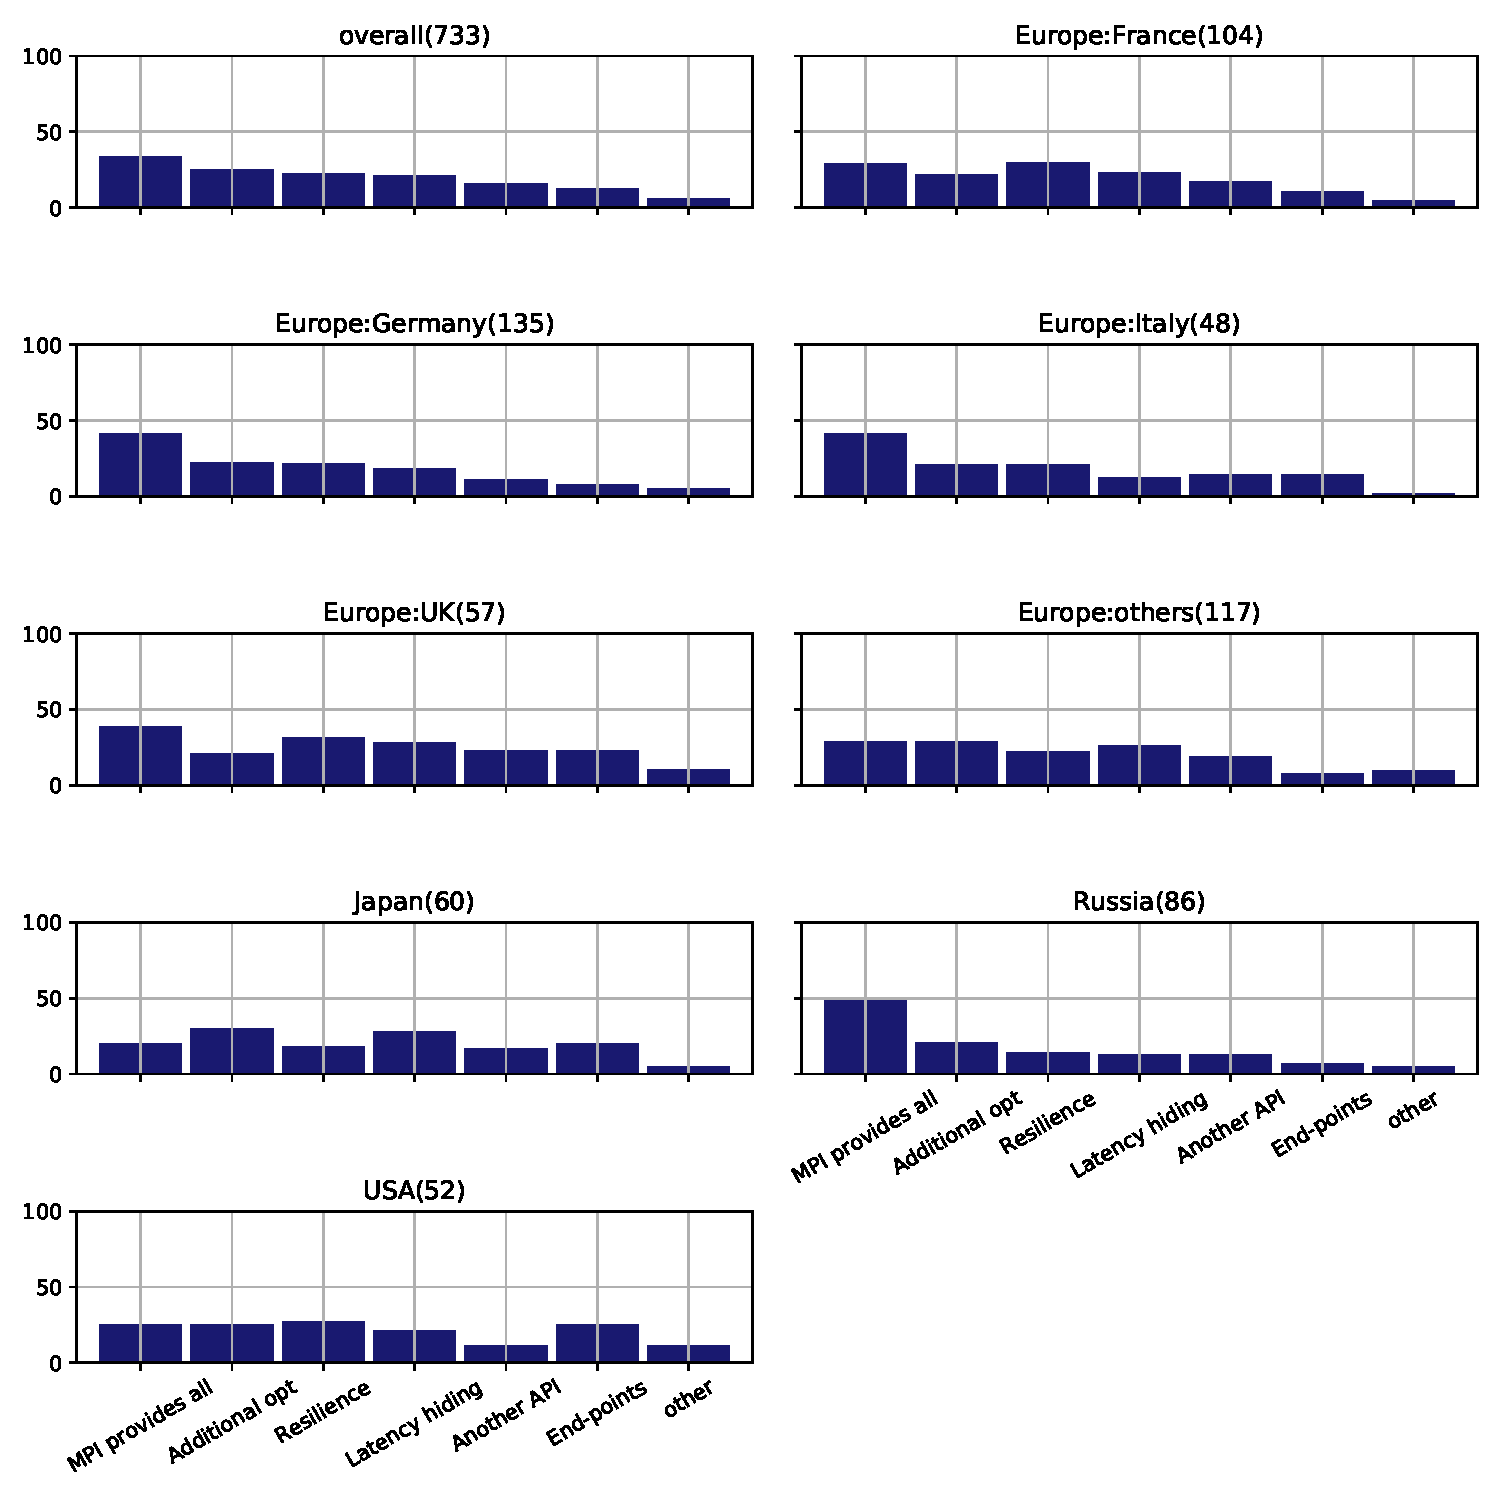
\includegraphics[width=10cm]{../pdfs/Q26.pdf}
\caption{Simple analysis: Q26}
\label{fig:Q26}
\end{center}
\end{figure}

\begin{figure}[htb]
\begin{center}
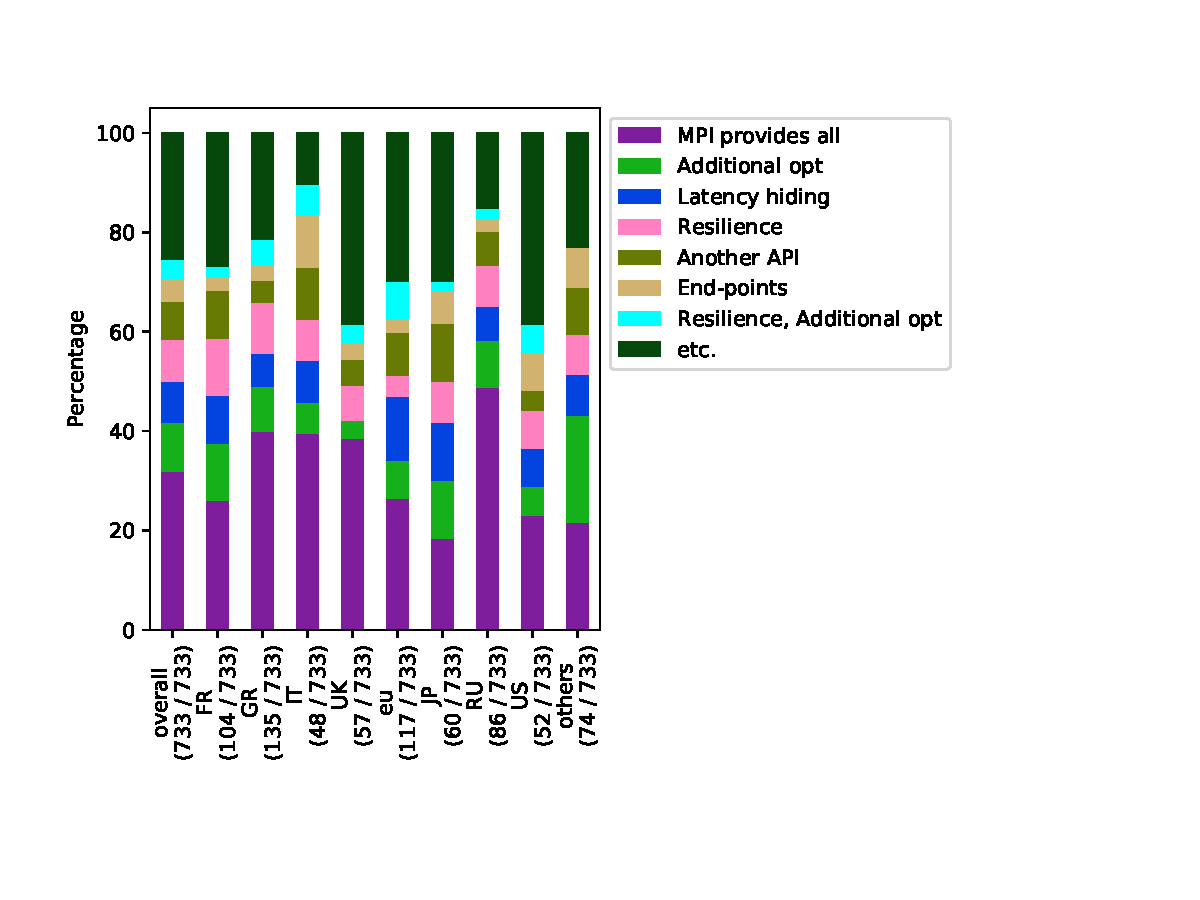
\includegraphics[width=14cm]{../pdfs/Q26-mans.pdf}
\caption{Multiple Answers: Q26}
\label{fig:Q26-mans}
\end{center}
\end{figure}
